\chapter{Thiết kế Facebook chatbot với Chatfuel}
\textit{Chatfuel} là một công cụ tạo chatbot miễn phí (cho quy mô nhỏ) giúp xây dựng nhanh một chatbot trên mạng xã hội Facebook. Chatfuel mạnh mẽ không chỉ ở giao diện trực quan, mà còn ở việc hỗ trợ JSON dành cho việc mở rộng thuật toán bằng lập trình.\par

\section{Nền tảng Chatfuel}
Để tạo chatbot với Chatfuel, trước hết cần có quyền \textit{quản trị viên} (administrator) của một trang Facebook (Facebook fanpage). Sau khi đăng nhập vào {\color{mTeal}\underline{dashboard.chatfuel.com}}, giao diện của Chatfuel tương tự như hình \ref{fig:fig-s3-1-chatfuel-dashboard}. Trong đó:
\begin{enumerate}[label=\textbf{(\arabic*)},align=left,left=0cm..0cm,itemindent=*]
	\item \textbf{Create from Template}: Tạo một chatbot mới từ mẫu có sẵn, hoặc một chatbot trắng.
	\item Menu xuất hiện ở các chatbot đã tạo cho phép thực hiện các thao tác cơ bản như \textit{đổi tên} (rename), \textit{sao chép} (copy), \textit{xóa} (delete).
	\item Chọn chatbot để truy cập giao diện làm việc chính của Chatfuel.
\end{enumerate}\par

\begin{figure}[htb!]\centering
	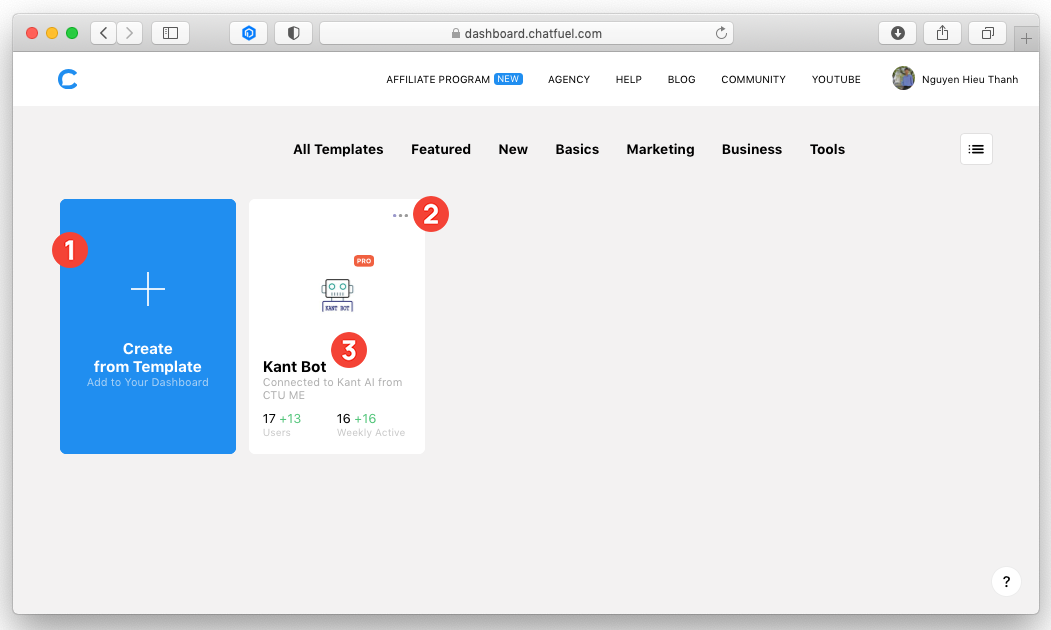
\includegraphics[width=15cm]{chatfuel/0-dashboard}
	\caption{Giao diện bắt đầu của Chatfuel}
	\label{fig:fig-s3-1-chatfuel-dashboard}
\end{figure}\par

\subsection{Giao diện làm việc}
Sau khi chọn chatbot, người dùng được chuyển tới giao diện làm việc của Chatfuel (hình \ref{fig:fig-s3-1-chatfuel-grow}), trước hết là mục \textit{Grow} – chứa các thông tin cơ bản để phát triển chatbot như \textit{trang Facebook đã kết nối} (connected page, mục \textbf{(8)}), cách bot trả lời lại một số tin nhắn người dùng thường gửi, các \textit{tiện ích mở rộng} (plugin).\par
\begin{figure}[htb!]\centering
	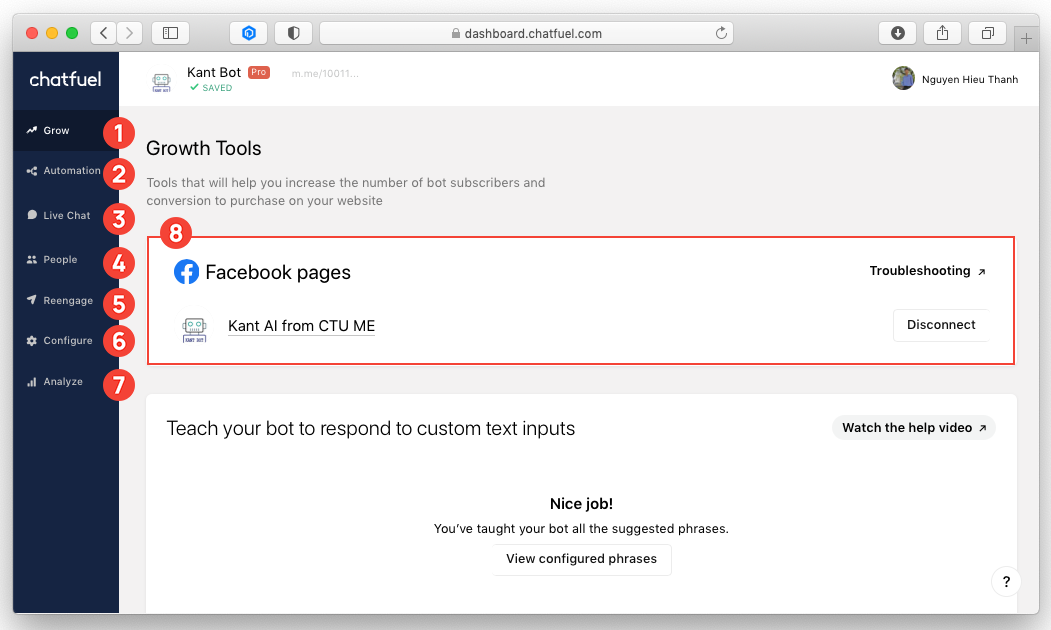
\includegraphics[width=15cm]{chatfuel/1-grow}
	\caption{Giao diện làm việc chính của Chatfuel}
	\label{fig:fig-s3-1-chatfuel-grow}
\end{figure}\par

Bên phải màn hình là thanh điều hướng:
\begin{enumerate}[label=\textbf{(\arabic*)},align=left,left=0cm..0cm,itemindent=*]
	\item \textbf{Grow}: Trang bắt đầu, chứa các thông tin cơ bản và công cụ giúp phát triển chatbot.
	\item \textbf{Automation}: Các thiết đặt trả lời tự động.
	\item \textbf{Live Chat}: Hiển thị các tin nhắn yêu cầu trò chuyện với quản trị viên (các vai trò trên chatbot được thiết đặt ở mục \textbf{(6)}).
	\item \textbf{People}: Hiển thị danh sách và các thuộc tính, thông tin người dùng đã tương tác với chatbot.
	\item \textbf{Re-engage}: Cho phép tương tác lại với các người dùng đã sử dụng chatbot, đã lâu không tương tác, chưa hoàn thành việc nào đó (theo điều kiện tự thiết đặt)...
	\item \textbf{Configure}: Cài đặt cho chatbot.
	\item \textbf{Analyze}: Các phân tích định lượng và gợi ý cho việc phát triển bot.
\end{enumerate}

\subsubsection{Mục Automation}
Phần này cung cấp các công cụ để tạo ra những cuộc hội thoại hoàn toàn tự động và linh hoạt (hình \ref{fig:fig-s3-2-chatfuel-automation-flows}):
\begin{enumerate}[label=\textbf{(\arabic*)},align=left,left=0cm..0cm,itemindent=*]
	\item \textbf{Flows}: Thiết đặt trả lời tự động thông qua các khối trực quan, việc này tương tự với biểu diễn thuật toán bằng biểu đồ.
	\item \textbf{Blocks}: Tạo ra các "khối" tin nhắn xác định, có thể dễ dàng di chuyển qua lại với Flows.
	\item \textbf{Set up AI}: Đặt các quy tắc trả lời tự động (hoặc chuyển hướng sang Block, Flow) thông qua việc nhận dạng các cụm từ, tin nhắn...
\end{enumerate}\par
\textbf{\textit{Flows}} cho phép sử dụng cấu trúc rẽ nhánh (nếu... thì...) và có thể điều hướng rất linh hoạt thông qua giao diện chỉnh sửa trực quan, do đó, nó thường được lựa chọn cho các cuộc hội thoại dài và phức tạp. Một flow có thể đảm nhiệm một mảng lớn của chatbot. Điển hình là các phần hướng dẫn, hỏi đáp (Q-A), khảo sát... Tuy nhiên, do vẫn còn ở giai đoạn thử nghiệm, nên flow vẫn chưa được hoàn thiện về mặt hiệu năng, đặc biệt là giao diện chỉnh sửa không ổn định khi làm việc với những flow mang tính phức tạp. Giao diện Flows gồm có hai phần: \textbf{(4)} danh sách các flow và \textbf{(5)} khu vực thiết kế flow với các nút lệnh \textbf{(6)} (hình \ref{fig:fig-s3-2-chatfuel-automation-flows}).\par

\begin{figure}[htb!]\centering
	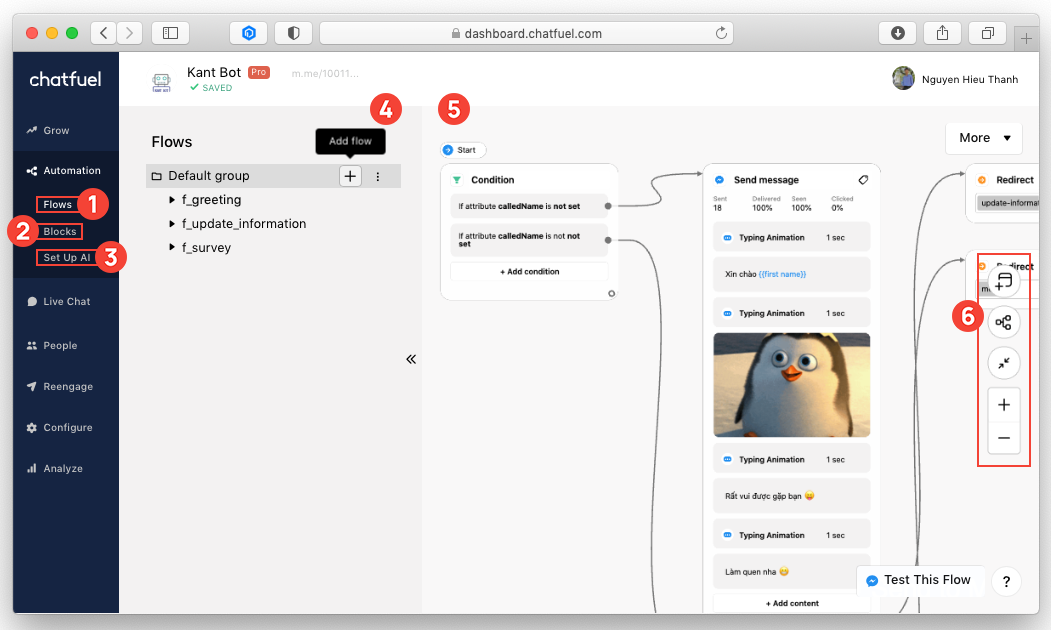
\includegraphics[width=15cm]{chatfuel/2-1-flows}
	\caption{Thiết đặt trả lời tự động với chức năng \textit{Flows}}
	\label{fig:fig-s3-2-chatfuel-automation-flows}
\end{figure}\par

\textbf{\textit{Blocks}} cho phép trả lời tự động thông qua các khối được thiết đặt từ trước. Blocks sử dụng giao diện chỉnh sửa tuyến tính và không hỗ trợ cấu trúc rẽ nhánh như Flows, nên một block không thể đảm nhận nhiều công việc. Khi chưa có flow, block thường được dùng riêng lẻ để gọi JSON API – thành phần quyết định các cấu trúc rẽ nhánh và điều hướng. Hiện nay, block thường được sử dụng cho các giao tiếp đơn giản, gửi các hình ảnh có sẵn, gọi JSON API cho các thuật toán phức tạp... Giao diện thiết lập block tương tự hình \ref{fig:fig-s3-2-chatfuel-automation-blocks}, trong đó: \textbf{(1)} chứ các nhóm và các block, \textbf{(2)} không gian biên tập block.\par
\begin{figure}[htb!]\centering
	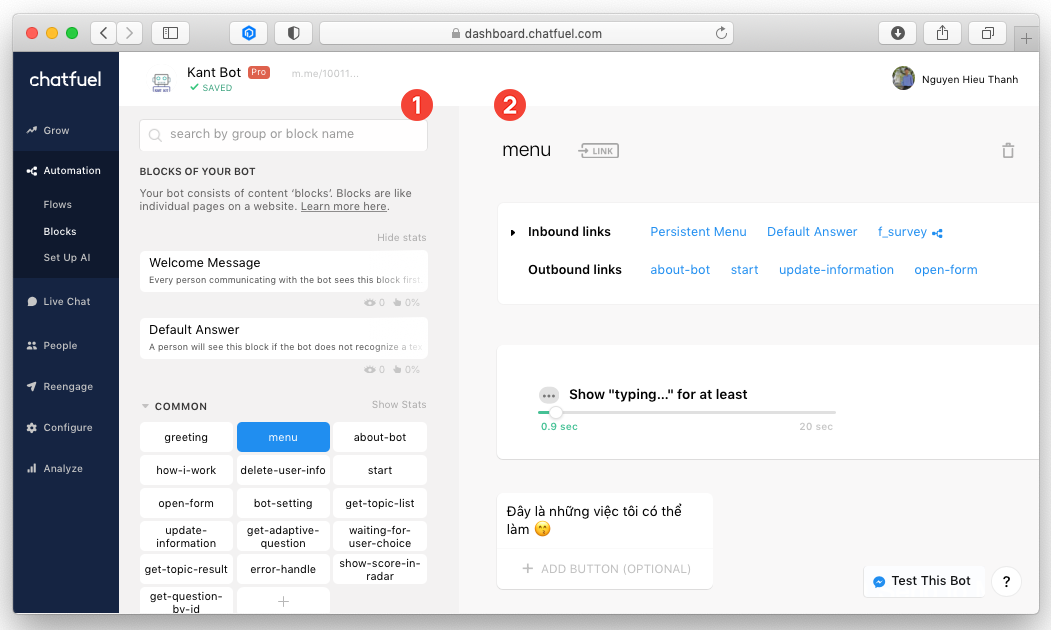
\includegraphics[width=15cm]{chatfuel/2-2-blocks}
	\caption{Thiết đặt trả lời tự động với chức năng \textit{Blocks}}
	\label{fig:fig-s3-2-chatfuel-automation-blocks}
\end{figure}\par

Phần \textbf{\textit{Set up AI}} cho phép kết hợp các flows và blocks lại với nhau, thông qua việc nhận dạng từ ngữ nhận được, bot sẽ trả lời bằng \textit{tin nhắn văn bản} (text messages) hoặc \textit{chuyển hướng} (re-direct) sang các phần khác. Ở phần này (hình \ref{fig:fig-s3-2-chatfuel-automation-ai}), người dùng có thể thêm mới một \textit{quy tắc} (rule – \textbf{(1)}), sau đó nhập các cụm từ vào mục \textbf{(2)} và thiết lập cách phản hồi của bot ở mục \textbf{(3)}.\par
\begin{figure}[htb!]\centering
	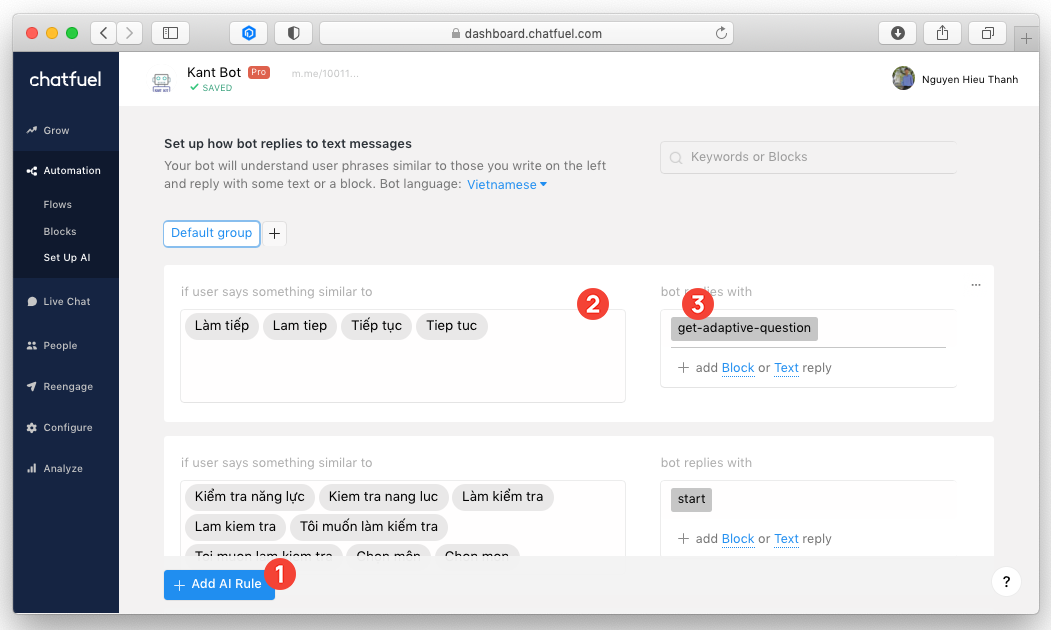
\includegraphics[width=15cm]{chatfuel/2-3-set-up-ai}
	\caption{Thiết đặt trả lời tự động với chức năng \textit{Set up AI}}
	\label{fig:fig-s3-2-chatfuel-automation-ai}
\end{figure}\par

Nếu sử dụng linh hoạt, ta hoàn toàn có thể tạo ra một chatbot tương tự người thật, với những khả năng được Chatfuel hỗ trợ:
\begin{itemize}
	\item Gửi hiệu ứng đang nhập tin nhắn.
	\item Gửi đi tin nhắn văn bản, hình ảnh, phim, âm thanh...
	\item Tạo một thư viện các sản phẩm, hình ảnh...
	\item Tạo ra các \textit{lựa chọn nhanh} (quick replies) cho phép người dùng trả lời nhanh.
	\item Lưu lại tin nhắn vừa nhận được.
	\item Thiết đặt các \textit{thuộc tính} (attribute) của người dùng.
\end{itemize}

\subsubsection{Mục People}
Mục people (hình \ref{fig:fig-s3-4-chatfuel-people}) cung cấp danh sách chi tiết người dùng đã tương tác với bot, các thuộc tính có sẵn và các thuộc tính tự thiết lập:
\begin{enumerate}[label=\textbf{(\arabic*)},align=left,left=0cm..0cm,itemindent=*]
	\item Hiển thị danh sách người dùng và các thuộc tính, thời gian truy cập... Phần này có thể tùy chỉnh danh sách các cột tùy theo nhu cầu sử dụng.
	\item Cung cấp chức năng lọc danh sách người dùng theo nhóm: người dùng chủ động nhắn tin với chatbot, người dùng nhấn vào quảng cáo, người dùng bình luận các bài đăng của fanpage...
	\item Quản lý chung danh sách người dùng của chatbot, cụ thể: lưu vào nhóm nào đó, xóa người dùng, xuất dưới dạng tệp CSV (Comma-separated values).
\end{enumerate}\par

\begin{figure}[htb!]\centering
	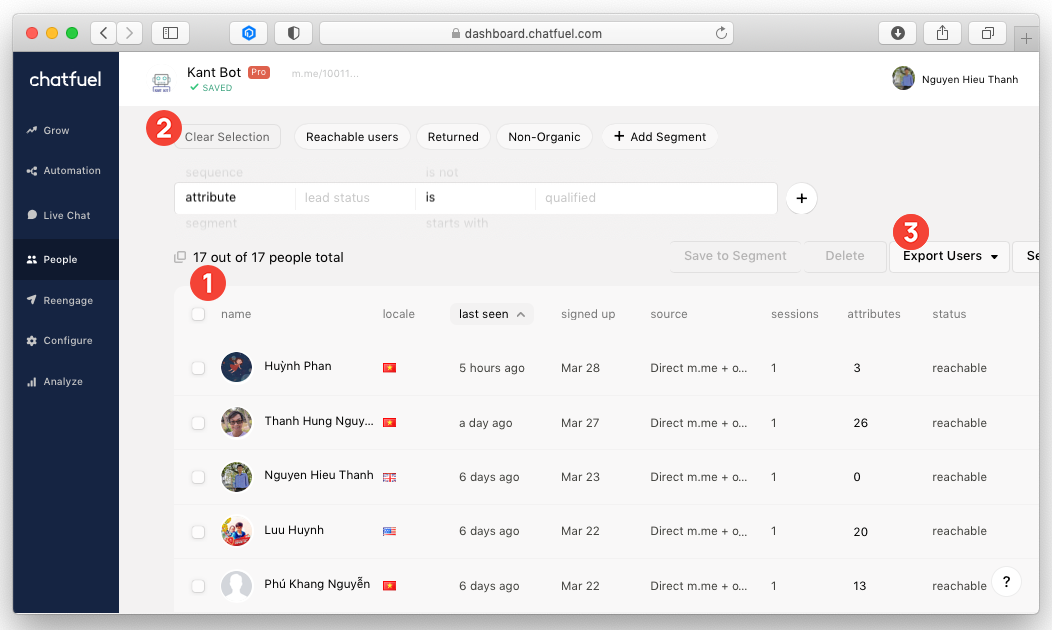
\includegraphics[width=15cm]{chatfuel/4-people}
	\caption{Giao diện danh sách người dùng đã tương tác với bot}
	\label{fig:fig-s3-4-chatfuel-people}
\end{figure}\par

\subsubsection{Mục Re-engage}
Chức năng này cung cấp nhiều cách để tương tác tự động với người dùng của bot. Chatfuel cho phép \textbf{(1)} gửi thủ công ngay lập tức, \textbf{(2)} lên lịch cho tin nhắn, \textbf{(3)} gửi tin nhắn theo một sự kiện được thiết lập sẵn (sau 24 giờ không tương tác, khi thay đổi một thuộc tính...), \textbf{(4)} tự động gửi tin nhắn từ các nguồn bên ngoài chatfuel (qua JSON API). Tin nhắn được thiết kế và gửi từ \textit{re-engage} hoàn toàn tương tự với giao diện thiết kế \textit{blocks} \textbf{(5)}.\par

\begin{figure}[htb!]\centering
	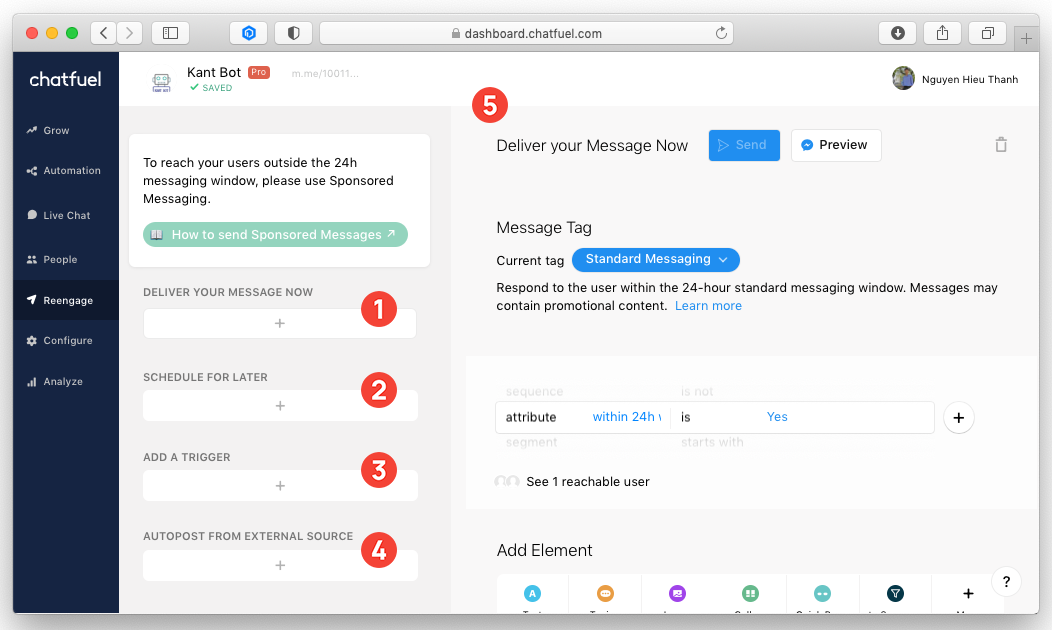
\includegraphics[width=15cm]{chatfuel/5-re-engage}
	\caption{Giao diện danh sách người dùng đã tương tác với bot}
	\label{fig:fig-s3-5-chatfuel-re-engage}
\end{figure}\par

